\chapter{Manual de usuario}

A continuación se explicarán las funcionalidades de la plataforma, apoyándose en capturas de pantalla del sistema.

\section{Página de inicio}

En la figura \ref{fig:man_inicio} se puede ver el aspecto que presenta la página de inicio de la plataforma. En la parte izquierda un menú desplegable permite navegar por los diferentes test que ofrece el sistema: evaluación de condiciones paramétricas, test paramétricos o no paramétricos.

\begin{figure}[H]
\centering
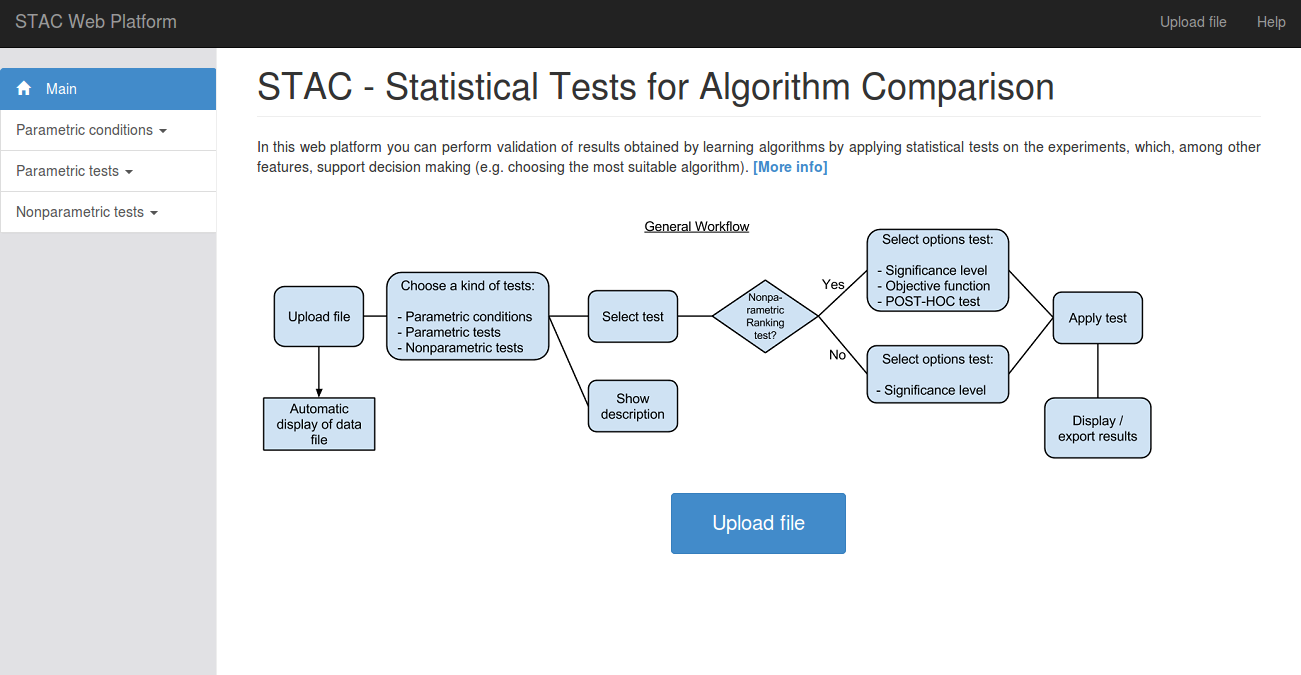
\includegraphics[scale=0.4]{figuras/man_inicio.png}
\caption{Página de inicio de la plataforma.}
\label{fig:man_inicio}
\end{figure}

Asimismo, y con la intención de que los usuarios no familiarizados con la plataforma se puedan hacer una idea de los pasos a seguir en la validación de resultados mediante los test, se muestra en la parte central de la ventana el flujo de trabajo a seguir en una sesión de uso de STAC. En la parte inferior, un botón para subir un fichero de datos resalta claramente como primer paso a realizar en la validación. En la figura \ref{fig:man_fichero} se puede ver la ventana emergente que se muestra para la subida de ficheros:

\begin{figure}[H]
\centering
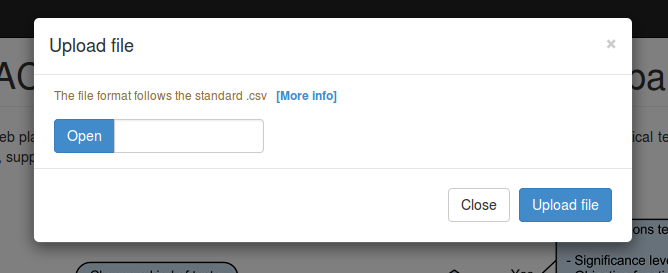
\includegraphics[scale=0.5]{figuras/man_fichero.png}
\caption{Ventana emergente de subida de ficheros.}
\label{fig:man_fichero}
\end{figure}

\begin{figure}[H]
\centering
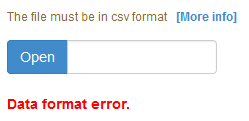
\includegraphics[scale=0.5]{figuras/man_fichero2.png}
\caption{Mensaje de error.}
\label{fig:man_fichero2}
\end{figure}

Para subir el fichero primero se debe hacer clic en ``Open", que abrirá la ventana de búsqueda del fichero. Para subir los datos, se debe hacer clic en ``Upload file". Asimismo, se puede cancelar la acción con ``Close", o haciendo clic en algún otro lugar de la plataforma distinto al de la ventana emergente para la subida de ficheros.

En la figura \ref{fig:man_fichero2}, se muestra un mensaje de error típico cuando los datos no cumplen con el formato especificado. Por otra parte, una barra de navegación superior (común a todas las páginas de la plataforma excepto en la página de ayuda) proporciona un botón de subida de ficheros, consulta de ficheros (después de realizar una subida) y acceso a la ayuda, de forma que desde cualquier página de la plataforma se pueda tanto subir y visualizar ficheros como ir directamente a la ayuda.

\section{Ayuda y consulta de datos}

Las figuras \ref{fig:man_ayuda1} y \ref{fig:man_ayuda2} representan algunas secciones de la ayuda y una sección en particular respectivamente (la del formato del fichero de datos):

\begin{figure}[H]
\centering
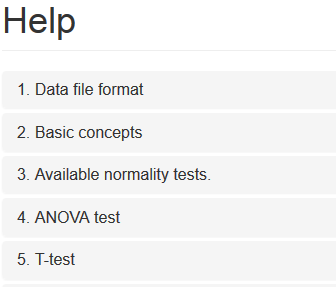
\includegraphics[scale=0.5]{figuras/man_ayuda1.png}
\caption{Listado secciones ayuda.}
\label{fig:man_ayuda1}
\end{figure}

A esta ayuda se accede, como se ha comentado anteriormente, a través de la barra de navegación superior. Sin embargo, la aplicación cuenta también con enlaces que permiten acceder directamente a secciones particulares de la ayuda. Como se puede apreciar en la ventana emergente de subida de ficheros (Fig. \ref{fig:man_fichero}), el enlace \texttt{[more info]} permite realizar esta acción, que nos llevaría a la página representada en la figura \ref{fig:man_ayuda2}. En toda la aplicación existen enlaces de este tipo (la mayoría de los cuales están dedicados a los test de la plataforma.)

\begin{figure}[H]
\centering
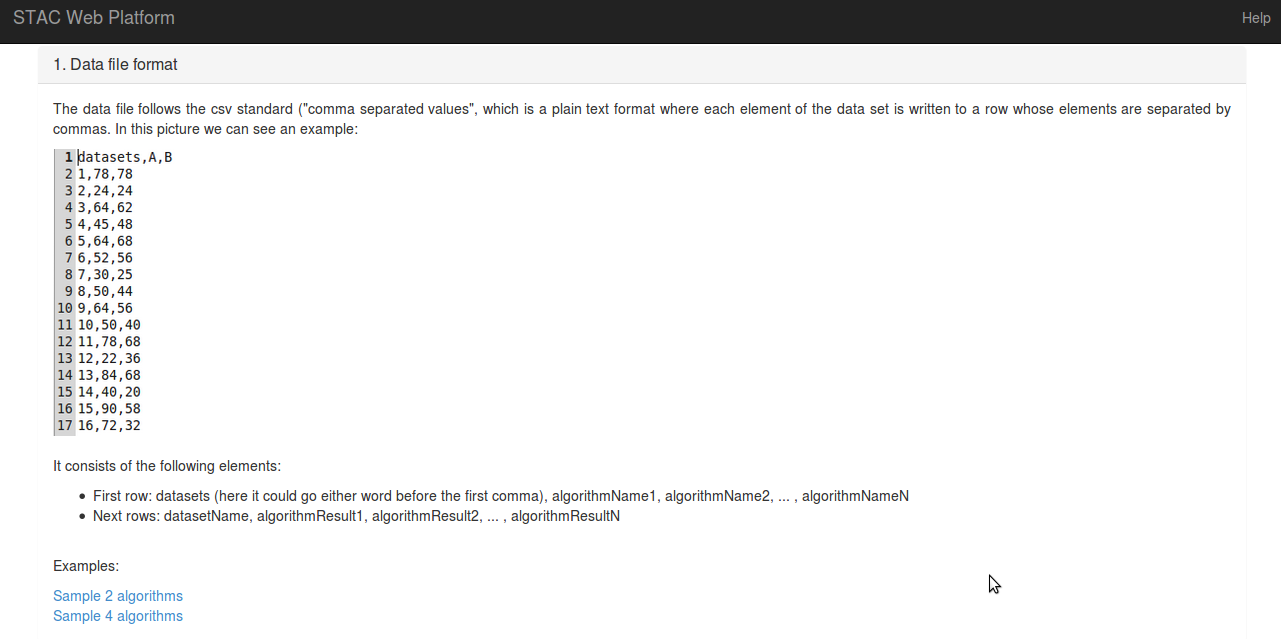
\includegraphics[scale=0.4]{figuras/man_ayuda2.png}
\caption{Sección del formato del fichero de datos.}
\label{fig:man_ayuda2}
\end{figure}

Por otra parte, en la figura \ref{fig:man_consulta} se muestra el aspecto de la pantalla de visualización del contenido del fichero. En esta pantalla, se resalta con un tono azul (similar al usado en los menús y botones del sistema) la línea de datos en la que está posicionado el ratón, con el fin de ayudar en la lectura.

\begin{figure}[H]
\centering
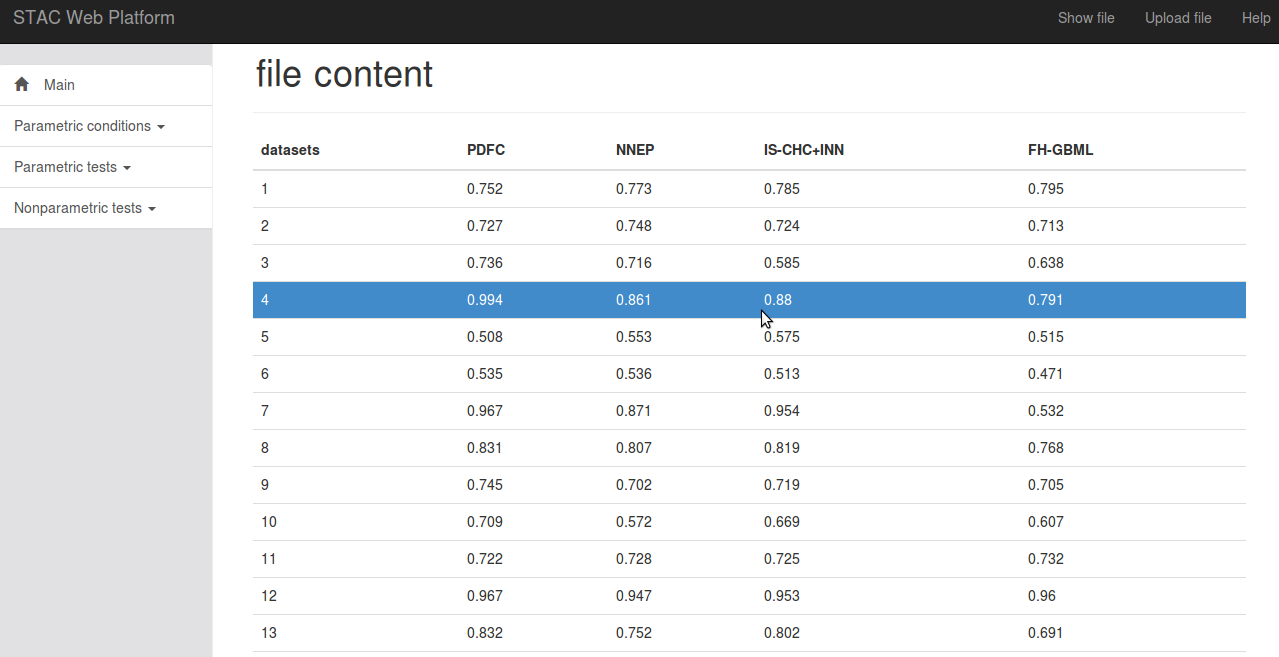
\includegraphics[scale=0.4]{figuras/man_consulta.png}
\caption{Pantalla de visualización del fichero de datos.}
\label{fig:man_consulta}
\end{figure}

\section{Selección de parámetros / opciones de test}

En cada sección en el menú desplegable de la izquierda (condiciones paramétricas, test paramétricos o no paramétricos) aparece como primera opción una descripción general de los test. Por ejemplo en la figura \ref{fig:man_descripcion} se puede ver la descripción de las condiciones paramétricas:

\begin{figure}[H]
\centering
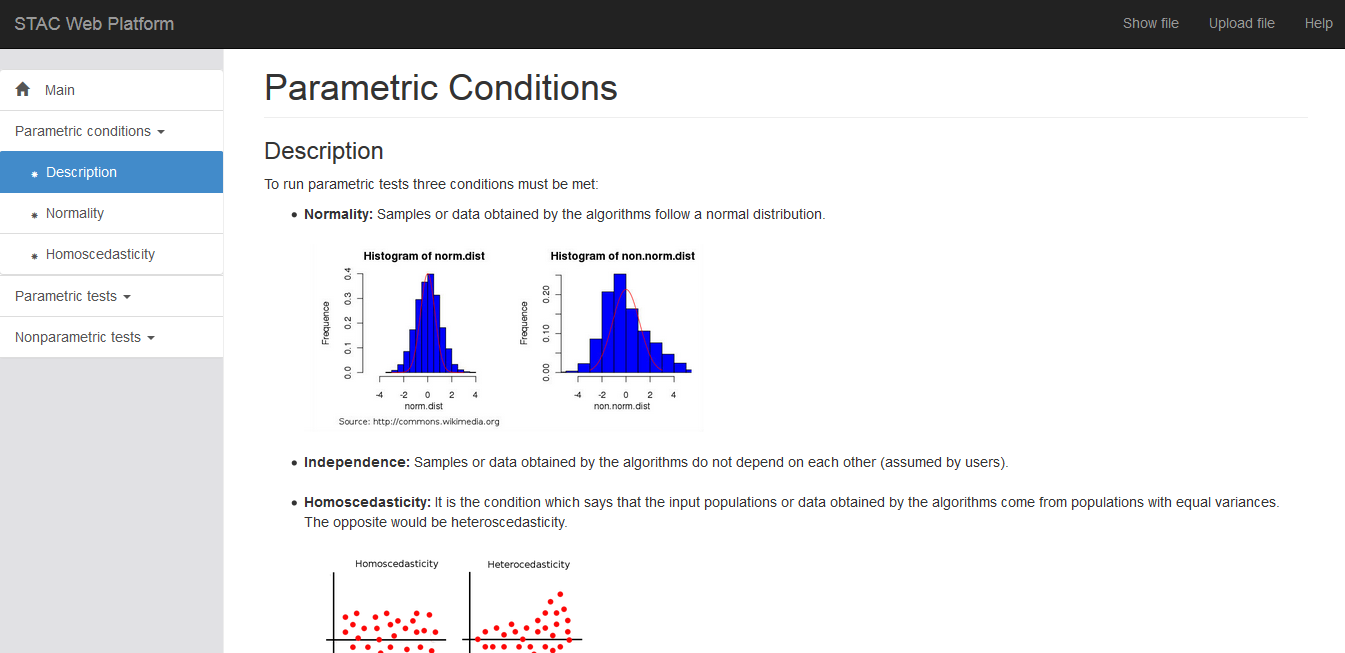
\includegraphics[scale=0.4]{figuras/man_descripcion.png}
\caption{Descripción de las condiciones paramétricas.}
\label{fig:man_descripcion}
\end{figure}

Cuando se selecciona un tipo de test determinado, la pantalla que se muestra permite la selección de un test en caso de que haya varios disponibles y sus opciones. Por ejemplo, en la figura \ref{fig:man_opciones} podemos ver las opciones disponibles para el caso de la sección de test de normalidad. En la parte superior disponemos de las distintas opciones. En la parte inferior se dispone de las descripciones, para que no interfieran en el proceso de aplicación de los test:

\begin{figure}[H]
\centering
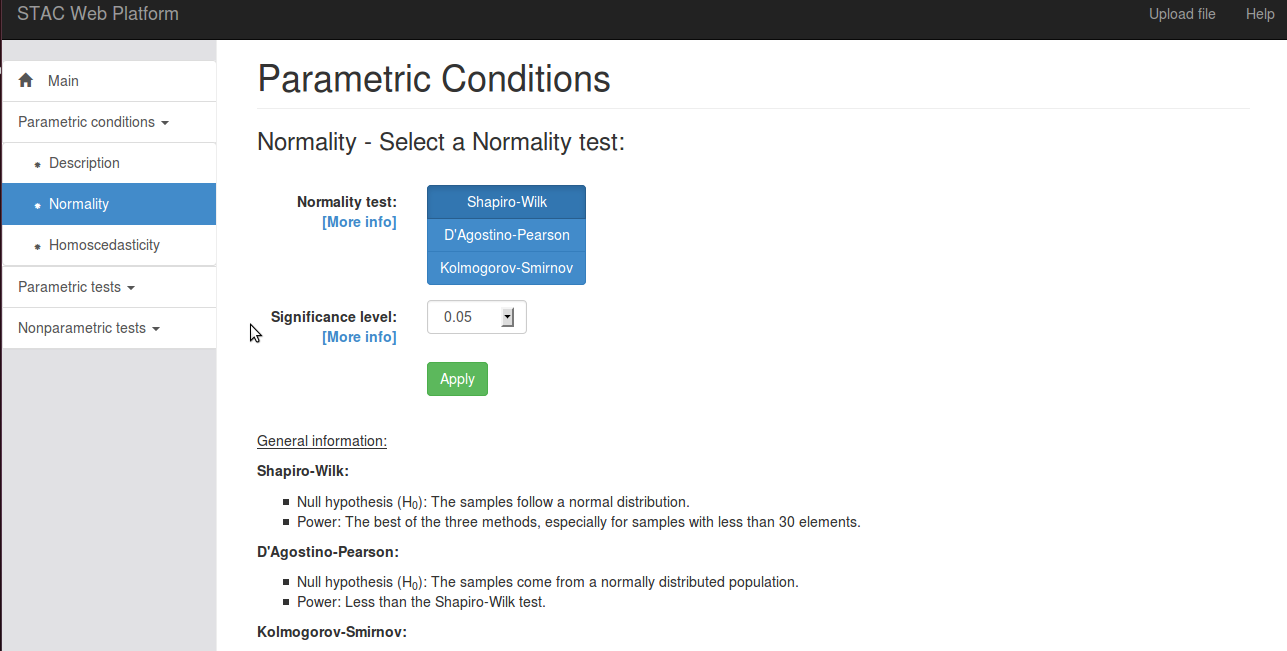
\includegraphics[scale=0.4]{figuras/man_opciones.png}
\caption{Selección de opciones.}
\label{fig:man_opciones}
\end{figure}

Como se puede ver, para cada opción existe un enlace directo a la sección de la ayuda que lo explica. Hay que destacar que no se puede aplicar ningún test en caso de que no exista un fichero de datos subido en la plataforma. En la figura \ref{fig:man_nofichero} se muestra el mensaje de error que se genera al querer aplicar un test sin datos. Por otra parte, ciertos test, como el T-Test o el test de Wilcoxon requieren únicamente ficheros de datos en los que sólo haya datos para dos algoritmos. Si se intenta aplicar estos test sobre ficheros con datos para más de dos algoritmos se genera un error como el que se muestra en la figura \ref{fig:man_errorapli}:

\begin{figure}[H]
\centering
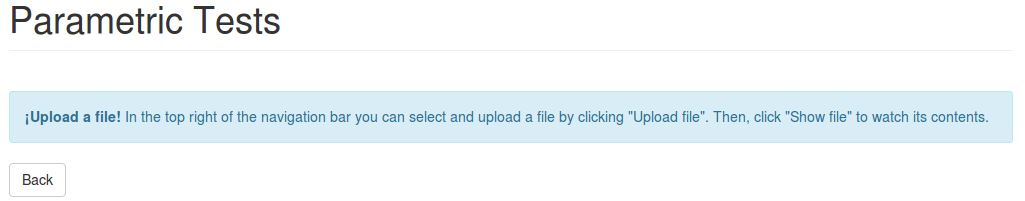
\includegraphics[scale=0.5]{figuras/man_nofichero.png}
\caption{Error cuando no existe ningún fichero.}
\label{fig:man_nofichero}
\end{figure}

\begin{figure}[H]
\centering
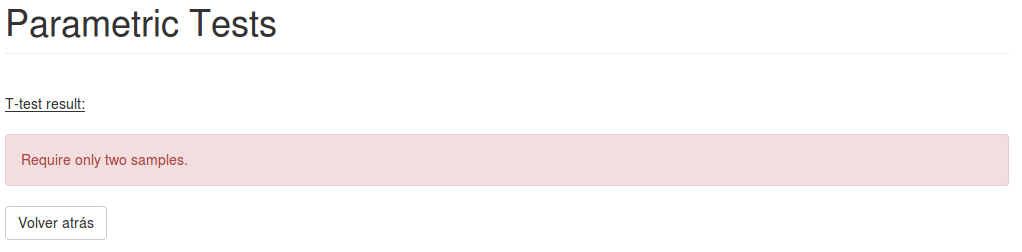
\includegraphics[scale=0.5]{figuras/man_errorapli.png}
\caption{Error cuando el número de algoritmos es mayor a 2.}
\label{fig:man_errorapli}
\end{figure}

También se muestran mensajes de aviso en caso de que se aplique un test paramétrico sin haber comprobado previamente si los datos cumplen con las condiciones paramétricas.

\section{Visualización de resultados}

Después de aplicar algún test, se muestra la pantalla con los resultados obtenidos representados en forma de tabla. En la figura \ref{fig:man_results} podemos ver la pantalla que se genera para mostrar los resultados. En este ejemplo en concreto se muestran los resultados obtenidos después de la aplicación de un test de ranking y un test POST-HOC, para los cuales se generan dos tablas:

\begin{figure}[H]
\centering
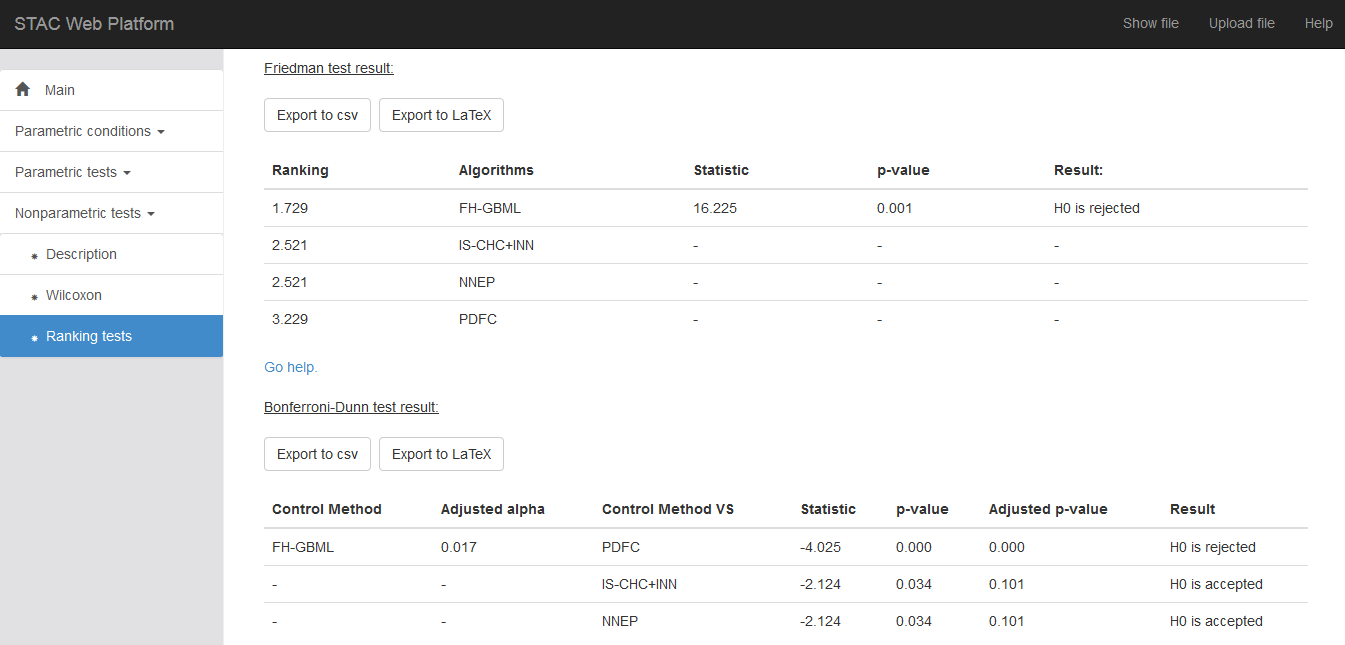
\includegraphics[scale=0.4]{figuras/man_results.png}
\caption{Página de visualización de resultados.}
\label{fig:man_results}
\end{figure}

Asimismo, en cada tabla se muestra la opción de exportar los resultados (tanto a formato \LaTeX \space como a formato CSV). Si se pulsa en uno de estos botones se abre una ventana de diálogo similar a la mostrada en la figura \ref{fig:man_dialog} para poder guardar el fichero generado:

\begin{figure}[H]
\centering
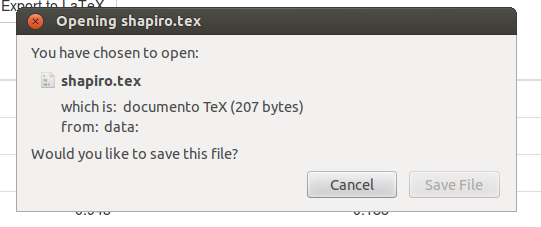
\includegraphics[scale=0.6]{figuras/man_dialog.png}
\caption{Ventana de diálogo exportación resultados.}
\label{fig:man_dialog}
\end{figure}

En las figuras \ref{fig:man_latex} y \ref{fig:man_csv} se muestra cómo sería el contenido de los resultados exportados (en \LaTeX \space y CSV respectivamente) para otro caso de ejemplo (resultados generados en la aplicación del test de normalidad de Shapiro-Wilk):

\begin{figure}[H]
\centering
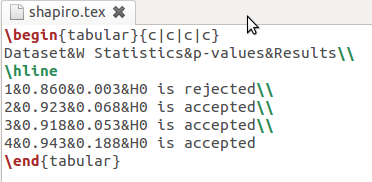
\includegraphics[scale=0.6]{figuras/man_latex.png}
\caption{Formato datos \LaTeX.}
\label{fig:man_latex}
\end{figure}

\begin{figure}[H]
\centering
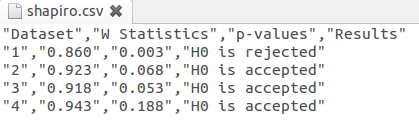
\includegraphics[scale=0.6]{figuras/man_csv.png}
\caption{Formato datos CSV.}
\label{fig:man_csv}
\end{figure}